\subsubsection*{La réécriture des évènements MIDI pour la batterie}
Basé sur \cite{jacquemard:hal-01134096} et sur \cite{jacquemard:hal-01403982}\\
Pour la plupart des instruments mélodiques, la liaison et le point sont les deux seules possibilités en cas d’équivalence rythmique pour des notes dont la durée de l’une à l’autre est ininterrompue. Mais puisque les durées des notes n’ont pas d’importance en batterie, l’usage des silences pour combler la distance rythmique entre deux notes devient possible.\\Les cymbales-crash et les ouvertures de charley constituent le seul cas qui exclut cette option. Le charley car ses ouvertures/fermetures sont presque toujours quantifiées et les cymbales-crash car elles peuvent être arrêtées à la main de manière quantifié aussi mais ce cas est très rare, nous allons donc nous concentrer sur les ouvertures de charley et considérer les crashs comme des événements sans durée.\\\\
Les fermetures du charley sont notées soit par un silence (correspondant à une fermeture de la pédale), soit par un écrasement de l’ouverture par un autre coup de charley fermé, au pied ou à la main.\\\\
\textbf{Exemples} :\\
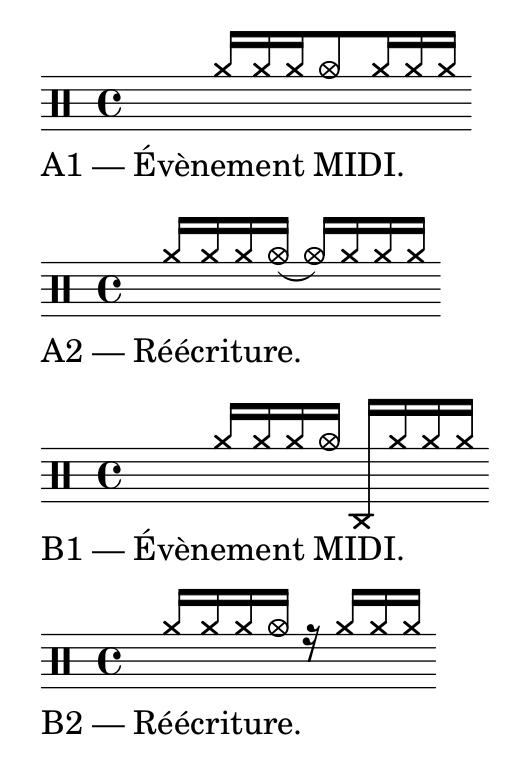
\includegraphics[height=80mm, width=60mm]{images/rewriting/exemples_charley_1.png}\\\\

\textbf{Exemples à écrire en arbre :}\\
\begin{itemize}
	\item 
	SI (pas pf) ET (note sur un temps suivie de note en l’air) :\\
	$\Rightarrow$ (Temps1 : Note pertinente) + (Temps2 : Silence pertinent + Note pertinente.)\\
	\item
	Si (po ou co) déborde sur le temps suivant :\\
	$\Rightarrow$ Liaison car marchera dans tous les cas même la où le point ne marchera pas (voir A2).\\
	\item
	Une blanche sera écrite noir + soupir.\\\\
\end{itemize}
\subsubsection{Les régles de réécriture}
~~\\
\Tree[.$\frac{2}{8}$ [.x ][.tie ]]\Tree[.2/8 [.x ]]\\\\\\
\Tree[.1/4 [.x ][.tie ]]\Tree[.1/4 [.x ][.r ]]\\\\\\